\documentclass[a4paper,11pt,fleqn]{article}%fleqn pour aligner les equations à gauche
\usepackage{../../Styles/Cours}

\newcommand{\chnum}{Chapitre 5}
\newcommand{\chtitle}{Cortège électronique}
\newcommand{\dtype}{Cours}

\usepackage{arydshln}%pour des ligne tableau en pointillé

\begin{document}
	\maketitle
\noindent\fbox{\begin{minipage}{.49\textwidth}
		\textbf{Document 1 : Le cortège électronique}\\
		L'ensemble des électrons d'un atome ou d'un ion est appelé \textbf{cortège électronique}. Il n'est pas possible de connaître la position exacte des électrons se déplaçant autour du noyau, cependant on peut connaître la probabilité de leur présence dans des zones appelées \textbf{couches électroniques}.
		\end{minipage}
		\begin{minipage}{.49\textwidth}
		\centering
		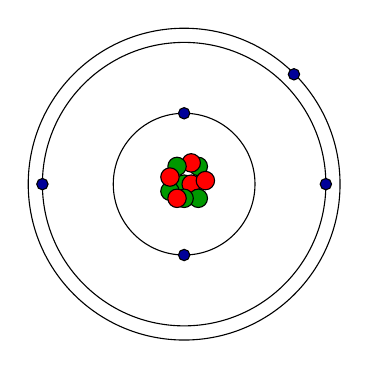
\begin{tikzpicture}[scale=.9, transform shape]
		\draw (0,0) circle (1);
		\draw (0,0) circle (2);
		\draw (0,0) circle (2.2);
		
		\draw[fill = green!60!black] (0,0) circle (.13);
		\draw[fill = red] (.1,0) circle (.13);
		\draw[fill = green!60!black] (.2,.25) circle (.13);
		\draw[fill = red] (.1,.3) circle (.13);
		\draw[fill = green!60!black] (-.1,.25) circle (.13);
		\draw[fill = green!60!black] (-.2,-.1) circle (.13);
		\draw[fill = red] (-.2,.1) circle (.13);
		\draw[fill = green!60!black] (.2,-.2) circle (.13);
		\draw[fill = red] (.3,.05) circle (.13);
		\draw[fill = green!60!black] (.0,-.2) circle (.13);
		
		\draw[fill = red] (-.1,-.2) circle (.13);
		
		\draw[fill = blue!60!black] (0,1) circle (.08);
		\draw[fill = blue!60!black] (0,-1) circle (.08);
		
		\draw[fill = blue!60!black] (2,0) circle (.08);
		\draw[fill = blue!60!black] (-2,0) circle (.08);
		
		\draw[fill = blue!60!black] (1.55,1.55) circle (.08);
		\end{tikzpicture}
		\begin{center}
			Représentation schématique des électrons autour de l'atome de Bore (\ce{^11_5B})
		\end{center}
\end{minipage}}

\noindent\fbox{\begin{minipage}{.49\textwidth}
		\textbf{Document 2 : Des couches concentriques}\\
		Les électrons sont répartis dans des couches $n$ (1, 2, 3, ...) puis dans des sous couches (s, p, ...). Les couches et sous couches ne peuvent contenir qu'un nombre maximal d'électrons :
		\begin{itemize*}
			\item 2 électrons maximum pour la sous couche $s$
			\item 6 électrons maximum pour la sous couche $p$
		\end{itemize*}
	Il faut remplir toute une couche avant de pouvoir passer à la suivante.\\
	La \textbf{configuration électronique correspond à la distribution des électrons}  correspond à la distribution des électrons du cortège électronique dans les différentes couches et sous couches. On remplit chaque sous couche avent de passer à la couche suivante. La configuration électronique se note de la manière suivante :
		\end{minipage}
		\begin{minipage}{.49\textwidth}
	\begin{tabular}{|c|c|>{\centering\arraybackslash}m{3.5cm}|} \hline
	\textbf{Couche}	& \textbf{Sous-couche} & \textbf{Nombre maximal d'électrons}\\ \hline
	\textbf{1} & \textbf{s} & \textbf{2}\\ \hline
	\multirow{2}{*}{\textbf{2}} & \textbf{s} & \textbf{2} \\ \cline{2-3}
	& \textbf{p} & \textbf{6} \\ \hline
	\multirow{2}{*}{\textbf{3}} & \textbf{s} & \textbf{2} \\ \cline{2-3}
	& \textbf{p} & \textbf{6}\\ \hline
	
	\end{tabular}
\end{minipage}}

\noindent \fbox{\begin{minipage}{.985\textwidth}
		\textbf{Document 3 : Couche de valence}\\
		Lorsque deux atomes ou deux ions se rapprochent, ce sont leur couche la plus externe qui sont en contact. Cette couche est appelée couche de \textbf{valence}. C'est le nombre d'électrons situés sur la couche de valence qui va déterminer les propriétés chimiques d'un atome ou d'un ion.
\end{minipage}}

\noindent \fbox{\begin{minipage}{.985\textwidth}
		\textbf{Document 4 : Propriétés chimiques ?}\\
		Le tableau périodique des éléments, ou tableau de Mendeleïev, range et classe les éléments chimiques par ordre croissant du nombre de protons ($Z$). Sa structure est établie en fonction de la configuration électronique des atomes :
		\begin{itemize*}
			\item Le numéro de chaque ligne correspond à une couché électronique maximale pour l'atome
			\item Les éléments d'une même colonne ont le même nombre d'électrons sur sa couche de valence.
		\end{itemize*}
\end{minipage}}

\noindent \colorbox{gray!10}{\begin{minipage}{.97\linewidth}
		\textbf{Document 5 : Exemple de l'aluminium}\\
		L'aluminium a l'écriture symbolique \ce{^27_13Al}. L'atome d'aliminium a 13 protons, donc 13 électrons. Ces électrons auront donc la configuration suivante :
		\begin{Large}
			$$\text{L'aluminium [\ce{_13Al}] : } \textcolor{red}{1}s^{\textcolor{orange}{2}} ~\textcolor{olive}{2}s^{\textcolor{orange}{2}}~\textcolor{olive}{2}p^{\textcolor{purple}{6}} \colorbox{blue!30}{$\textcolor{blue}{3}s^{\textcolor{orange}{2}}~\textcolor{blue}{3}p^{\textcolor{purple}{1}}$}$$
		\end{Large}
		L'aluminium se situe à la troisième ligne (3 couches) du tableau et à la troisième colonne (3 électrons du sa couche de valence)	
\end{minipage}}

\begin{table}[h!]
\small \centering 
\caption{Tableau périodique simplifié}
\begin{tabular}{|c|c|c|c:c|c|c|c|c|c|c|}
		\cline{1-3}\cline{6-11} & 1 & 2 & & & 13 & 14 & 15 & 16 & 17 & 18\\
		\cline{1-3}\cline{6-11} 1 & \textbf{\ce{^1_1He}}& & & & & & & & & \textbf{\ce{^4_2He}}\\
		&Hydrogène& & & & & & & & & Hélium\\
		
		\cline{1-3}\cline{6-11} 2 & \textbf{\ce{^7_3Li}}& \textbf{\ce{^9_4Be}} & & & \textbf{\ce{^11_5B}}&\textbf{\ce{^12_6C}} &\textbf{\ce{^14_7N}} & \textbf{\ce{^16_8O}}&\textbf{\ce{^19_9F}} & \textbf{\ce{^20_10Ne}}\\
		&Lithium & Béryllium & & & Bore & Carbone & Azote & Oxygène & Fluor & Néon\\
		
		\cline{1-3}\cline{6-11} 3 & \textbf{\ce{^23_11Na}}& \textbf{\ce{^24_12Mg}} & & & \textbf{\ce{^27_13Al}}&\textbf{\ce{^28_14Si}} &\textbf{\ce{^31_15P}} & \textbf{\ce{^32_16S}}&\textbf{\ce{^25_17Cl}} & \textbf{\ce{^40_18Ar}}\\
		&Sodium & Magnésium & & & Aluminium & Silicium & Phosphore & Soufre & Chlore & Argon\\
		\cline{1-3}\cline{6-11}		
	\end{tabular}

\end{table}

\noindent\textbf{Question : le sodium est un élément chimique qui, sous sa forme solide, est très réactif au contact de l'eau. En se basant sur les documents précédents, comment va réagir le lithium une fois plongé dans l'eau ?}


\end{document}